\begin{frame}
  \frametitle{Användargränssnitt}
  \framesubtitle{foo}
  \begin{figure}
    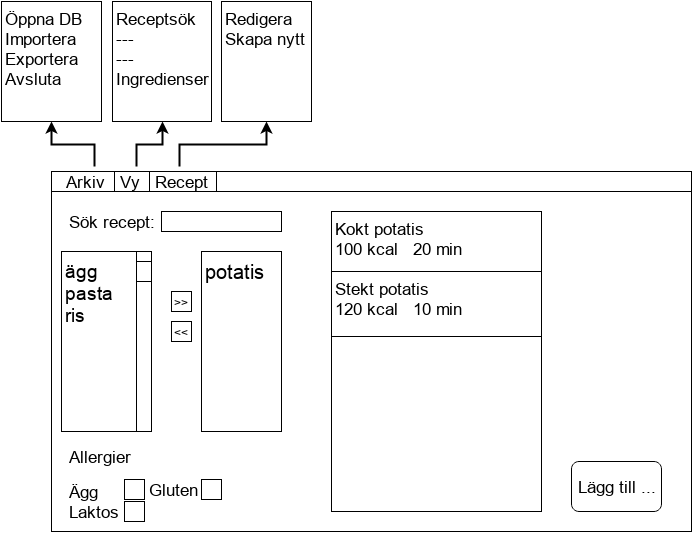
\includegraphics[scale=.33]{vy1}
  \end{figure}
  \begin{itemize}
    \item text här
  \end{itemize}
\end{frame}

\begin{frame}
  \frametitle{Användargränssnitt}
  \framesubtitle{foo}
  \begin{figure}
    
\includegraphics[scale=.4]{vy2}
  \end{figure}
  \begin{itemize}
    \item text här
  \end{itemize}
\end{frame}

\begin{frame}
  \frametitle{Användargränssnitt}
  \framesubtitle{foo}
  \begin{figure}
    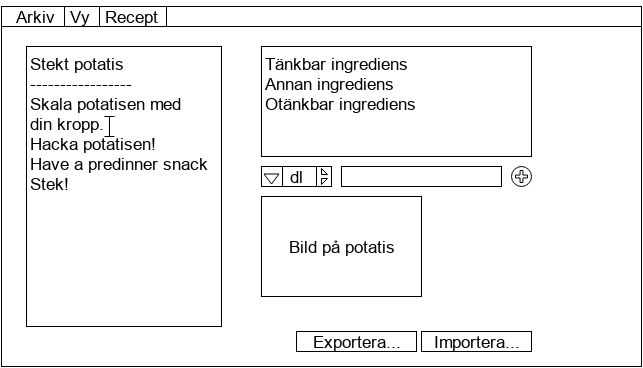
\includegraphics[scale=.4]{vy3}
  \end{figure}
  \begin{itemize}
    \item text här
  \end{itemize}
\end{frame}

\begin{frame}
  \frametitle{Användargränssnitt}
  \framesubtitle{foo}
  \begin{figure}
    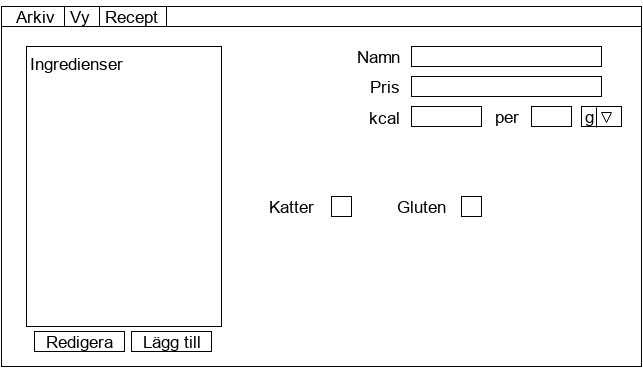
\includegraphics[scale=.4]{vy4}
  \end{figure}
  \begin{itemize}
    \item text här
  \end{itemize}
\end{frame}


